\section{Discussion}
\label{subsec:qualitative-eval}

In this section, we address requirement R1 by showing insights on the work history of files that are related. To this end we focused on the project \emph{smsr}, which has 21 commits over a time span of ten days.

%\todo[inline]{an example where it succeds:}
%\subsubsection{Example of work dependencies.}
%\subsubsection{Example of correct discovery.}
%\label{subsub:example}
Let us consider an example where our technique proves helpful. Our technique finds 6 highly related pairs, as shown in \Cref{table:evaluation-results-new}. We excluded files that have a functional dependencies, e.g. interface-class relations, where a change in the interface trivially brings change in the class. Thus, we were able to select the files \texttt{smsr/running example/Requirements/requirements.txt} and \texttt{smsr/running example/Software/model.java}, having $\chi=0.7$ and $d=4$. Moreover, by observing the content we verified that they do not have functional dependencies. Therefore, these two files are work dependent.
\Cref{fig:evaluated-processes} shows the extracted processes after mining their stories. Interestingly, the two processes do not share any activity because they were never changed together in the same commit.
%Literature approaches that leverage on network analysis can not uncover these type of dependencies, which are instead visible by the time series analysis.

\begin{figure}[t]
	\begin{subfigure}[t]{\textwidth}
		\centering
		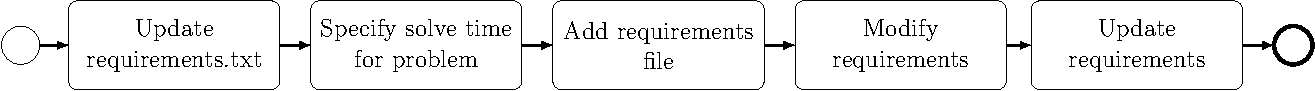
\includegraphics[width=.9\linewidth]{bpm2017/figures/six-processes/requirementsTxtProcess.pdf}
		\caption{Evolution of file \texttt{requirements.txt}}
		\label{subfig:requirements-file-process}
	\end{subfigure}
	\begin{subfigure}[ht]{\textwidth}
		\centering
		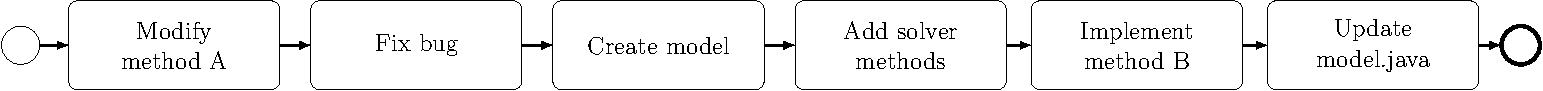
\includegraphics[width=.9\linewidth]{bpm2017/figures/six-processes/modelProcess.pdf}
		\caption{Evolution of file \texttt{model.java}}
		\label{subfig:model-file-process}
	\end{subfigure}
	\caption{Processes of two work-dependent files}
	\label{fig:evaluated-processes}
\end{figure}
%\todo[inline]{An example where it fails for some specific reason:}
%\subsubsection{Example of challenge.}

Our technique can fail under some circumstances. Consider the example above. We know that the files \texttt{requirements.txt} and \texttt{model.java} are work dependent. Let us now assume that the assumption of \emph{regular commits} in the \gls{vcs} does not hold. Nevertheless, we know that there is the following work pattern: \emph{at irregular times, one change in the requirements produces 2 changes of work that must be implemented in model in the next day}. In a short time window of 4 days, the time series would be $X_{req} = (1,0,1,0)$, $X_{model} = (0,2,0,2)$ and their correlation is $\sigma(f_{req},f_{model}) = -1$. Hence, they would score a high degree of co-evolution $\chi=1$. However, if we double the time window  and observe only another pattern the correlation would change. We get $X_{req} = (1,0,1,0,0,1,0,0)$, $X_{model} = (0,2,0,2,0,0,2,0)$ which score a $\sigma(f_{req},f_{model}) = -0.66$, $\chi=0.66$ and therefore not a high value of correlation.
%In these cases, approached that mine patterns of changes would outperform our approach.

These results show that our technique helps uncovering work dependencies that are not captured by existing approaches in literature which leverage on social network analysis~\cite{Zimmermann2008,Weicheng2013}. On the other hand, our technique is currently not yet able to retrieve dependencies with delay. We plan to address this challenge by using moving-average time series models. 